\section{Use-case diagram}

\begin{figure}[H]
    \centering
    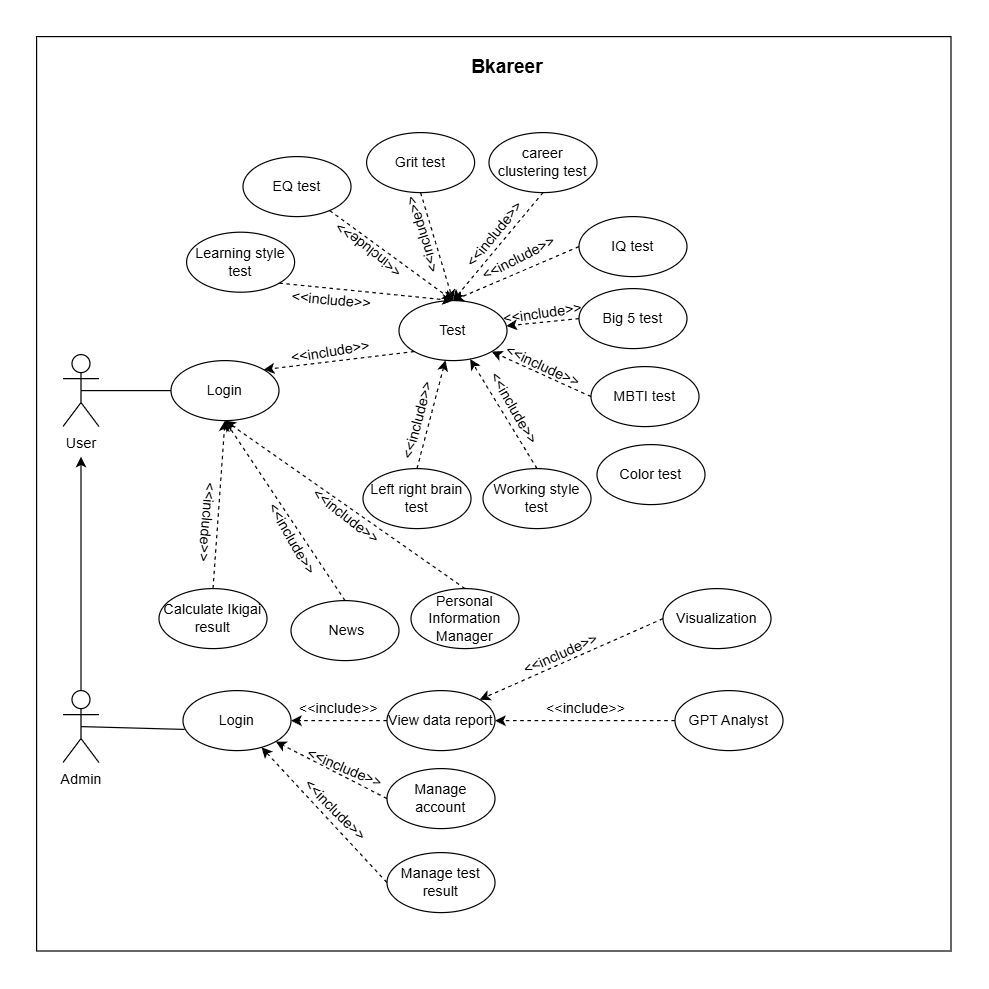
\includegraphics[width=0.5\linewidth]{images/usecase.png}
    \vspace{0.6cm}
    \caption{Use-case Diagram hệ thống}
\end{figure}

\subsection{Use-case Đăng nhập}
    \begin{longtable}[H]{|l|p{0.7\textwidth}|}
        \caption{Use-case Đăng nhập} \\
        \hline
        \textbf{Tên use-case} & Đăng nhập \\
    \hline
        \textbf{Actor} & Người dùng, quản trị viên \\
    \hline
        \textbf{Descriptions} & Cho phép người dùng đăng nhập vào hệ thống. \\
    \hline
        \textbf{Pre-conditions} & \vspace{-1cm} \begin{itemize}[leftmargin=4mm]
            \setlength\itemsep{0em}
            \item Hệ thống sẵn sàng để hoạt động.
            \item Người dùng đã có tài khoản.
        \end{itemize} \\
            
    \hline
        \textbf{Post-conditions} & \vspace{-1cm}  \begin{itemize} [leftmargin=4mm]
            \setlength\itemsep{0em}
            \item Người dùng đã đăng nhập thành công và có quyền truy cập vào hệ thống.
        \end{itemize} \\
    \hline
        \textbf{Normal Flow} & \vspace{-1cm} \begin{enumerate}[leftmargin=5.5mm]
            \setlength\itemsep{0em}
            \item Người dùng truy cập vào trang đăng nhập.
            \item Hệ thống hiển thị giao diện đăng nhập với các trường nhập thông tin: Tên đăng nhập và Mật khẩu.
            \item Người dùng nhập Tên đăng nhập và Mật khẩu của mình vào các trường tương ứng.
            \item Người dùng nhấn nút ``Đăng Nhập".
            \item Hệ thống kiểm tra thông tin đăng nhập của người dùng:
                \begin{itemize}
                    \item Nếu thông tin đăng nhập chính xác và hợp lệ:
                        \begin{itemize}
                            \item Hệ thống chuyển hướng người dùng đến trang chính của ứng dụng.
                            \item Người dùng được đăng nhập vào hệ thống và có thể sử dụng các chức năng.
                        \end{itemize}
                    \item Nếu thông tin đăng nhập không chính xác hoặc không hợp lệ:
                        \begin{itemize}
                            \item Hệ thống hiển thị thông báo lỗi cho người dùng, yêu cầu họ nhập lại thông tin đăng nhập.
                        \end{itemize}
                \end{itemize}
            \item Người dùng tiếp tục nhập lại thông tin đăng nhập hoặc thực hiện các hành động khác (đổi mật khẩu, quên mật khẩu,...).
        \end{enumerate} \\
    \hline
        \textbf{Alternative Flow} & Không có \\
    \hline 
        \textbf{Exception Flow} & \vspace{-1cm} \begin{enumerate}[leftmargin=5.5mm]
            \item Lỗi kết nối mạng
                \begin{itemize}[topsep=0pt]
                    \setlength\itemsep{0em}
                    \item Khi hệ thống không thể kết nối với máy chủ hoặc có sự cố về mạng.
                    \item Hệ thống hiển thị thông báo lỗi và yêu cầu người dùng thử lại sau khi có kết nối mạng ổn định.
                \end{itemize}
            \item Lỗi hệ thống:
                \begin{itemize}[topsep=0pt]
                    \setlength\itemsep{0em}
                    \item Khi hệ thống gặp sự cố hoặc lỗi nội bộ.
                    \item Hệ thống ghi lại lỗi và hiển thị thông báo lỗi cho người dùng.
                    \item Người dùng được khuyến nghị liên hệ với quản trị viên hoặc bộ phận hỗ trợ kỹ thuật để giải quyết vấn đề.
                \end{itemize}
        \end{enumerate}\\
    \hline 
    \end{longtable}

\subsection{Use-case Đăng Ký}
    \begin{longtable}[H]{|l|p{0.7\textwidth}|}
        \caption{Use-case Đăng Ký}
        \\ \hline
        \textbf{Tên use-case} & Đăng Ký \\
        \hline
        \textbf{Actor} & Người dùng, quản trị viên \\
        \hline
        \textbf{Descriptions} & Cho phép người dùng đăng ký tài khoản trên hệ thống. \\
        \hline
        \textbf{Pre-conditions} & \vspace{-1cm} \begin{itemize}[leftmargin=4mm]
            \setlength\itemsep{0em}
            \item Hệ thống sẵn sàng để hoạt động.
        \end{itemize} \\
            
        \hline
    
        \textbf{Post-conditions} & \vspace{-1cm}  \begin{itemize} [leftmargin=4mm]
            \setlength\itemsep{0em}
            \item Người dùng đã đăng ký thành công.
        \end{itemize} \\
                
        \hline
            
        \textbf{Normal Flow} & \vspace{-1cm} \begin{enumerate}[leftmargin=5.5mm]
            \setlength\itemsep{0em}
            \item Người dùng truy cập vào trang đăng ký.
            \item Hệ thống hiển thị giao diện đăng ký với các trường nhập thông tin: Tên người dùng, Địa chỉ email, Mật khẩu, Xác nhận mật khẩu.
            \item Người dùng nhập thông tin cá nhân vào các trường tương ứng.
            \item Người dùng nhấn nút ``Đăng Ký".
            \item Hệ thống kiểm tra tính hợp lệ của thông tin đăng ký:
                \begin{itemize}
                    \setlength\itemsep{0em}
                    \item Nếu thông tin đăng ký hợp lệ:
                        \begin{itemize}
                            \setlength\itemsep{0em}
                            \item Hệ thống tạo một tài khoản mới cho người dùng trong cơ sở dữ liệu.
                            \item Người dùng được chuyển hướng đến trang đăng nhập để đăng nhập vào tài khoản mới được tạo.
                        \end{itemize}
                    \item Nếu thông tin đăng ký không hợp lệ hoặc trùng lặp với thông tin đã tồn tại:
                        \begin{itemize}
                            \setlength\itemsep{0em}
                            \item Hệ thống hiển thị thông báo lỗi cho người dùng và yêu cầu họ nhập lại thông tin đăng ký.
                        \end{itemize}
                \end{itemize}
        \end{enumerate}\\
            
        \hline
            
        \textbf{Alternative Flow} & Không có \\
            
        \hline 
            
        \textbf{Exception Flow} & \vspace{-1cm} \begin{enumerate}[leftmargin=5.5mm]
            \item Lỗi kết nối mạng
                \begin{itemize}[topsep=0pt]
                    \setlength\itemsep{0em}
                    \item Khi hệ thống không thể kết nối với máy chủ hoặc có sự cố về mạng.
                    \item Hệ thống hiển thị thông báo lỗi và yêu cầu người dùng thử lại sau khi có kết nối mạng ổn định.
                \end{itemize}
            \item Lỗi hệ thống:
                \begin{itemize}[topsep=0pt]
                    \setlength\itemsep{0em}
                    \item Khi hệ thống gặp sự cố hoặc lỗi nội bộ.
                    \item Hệ thống ghi lại lỗi và hiển thị thông báo lỗi cho người dùng.
                    \item Người dùng được khuyến nghị liên hệ với quản trị viên hoặc bộ phận hỗ trợ kỹ thuật để giải quyết vấn đề.
                \end{itemize}
        \end{enumerate}\\
        \hline 
    \end{longtable}
    
\subsection{Use-case Xem thông tin giáo dục}
    \begin{longtable}[H]{|l|p{0.7\textwidth}|}
        \caption{Use-case Xem thông tin giáo dục}
        \\ \hline
        \textbf{Tên use-case} & Xem thông tin giáo dục \\
        \hline
        \textbf{Actor} & Người dùng \\
        \hline
        \textbf{Descriptions} & Chức năng này cung cấp các thông tin về các ngành đại học, các trường đại học, các hội thảo giáo dục, được cập nhật liên tục. \\
        \hline
        \textbf{Pre-conditions} & \vspace{-1cm} \begin{itemize}[leftmargin=4mm]
            \setlength\itemsep{0em}
            \item Hệ thống sẵn sàng để hoạt động.
            \item Người dùng đã đăng nhập vào hệ thống.
        \end{itemize} \\
        
        \hline

        \textbf{Post-conditions} & \vspace{-1cm} \begin{itemize}[leftmargin=4mm]
            \setlength\itemsep{0em}
            \item Người dùng đã truy cập và xem được thông tin về các ngành đại học, các trường đại học, các hội thảo giáo dục.
        \end{itemize} \\
            
        \hline
        
        \textbf{Normal Flow} & \vspace{-1cm} 
                \begin{enumerate}[leftmargin=5.5mm]
                    \setlength\itemsep{0em}
                    \item Người dùng truy cập vào phần "Tin tức" trên giao diện của hệ thống.
                    \item Hệ thống hiển thị danh sách các tin tức liên quan đến giáo dục, các trường đại học, các hội thảo giáo dục.
                    \item Người dùng có thể xem chi tiết thông tin về mỗi mục bằng cách nhấp vào từng mục.
                    \item Sau khi xem thông tin, người dùng có thể quay lại trang Tin tức hoặc thoát khỏi trang. 
                \end{enumerate}\\
                
        \hline
        
        \textbf{Alternative Flow} & \vspace{-1cm}  \begin{itemize}[leftmargin=4mm]
            \setlength\itemsep{0em}
            \item Không có thông tin nào được hiển thị: Nếu không có thông tin nào được cập nhật, hệ thống sẽ hiển thị thông báo ``Không có thông tin nào được tìm thấy" và người dùng có thể quay lại hoặc thoát.
        \end{itemize} \\
        
        \hline
        
        \textbf{Exception Flow} & \vspace{-1cm}  \begin{enumerate}[leftmargin=5.5mm]
            \setlength\itemsep{0em}
            \item Lỗi kết nối mạng
                \begin{itemize}
                    \setlength\itemsep{0em}
                    \item Khi hệ thống không thể kết nối với máy chủ hoặc có sự cố về mạng.
                    \item Hệ thống hiển thị thông báo lỗi và yêu cầu người dùng thử lại sau khi có kết nối mạng ổn định.
                \end{itemize}
            \item Lỗi hệ thống:
                \begin{itemize}
                    \setlength\itemsep{0em}
                    \item Khi hệ thống gặp sự cố hoặc lỗi nội bộ.
                    \item Hệ thống ghi lại lỗi và hiển thị thông báo lỗi cho người dùng.
                    \item Người dùng được khuyến nghị liên hệ với quản trị viên hoặc bộ phận hỗ trợ kỹ thuật để giải quyết vấn đề.
                \end{itemize}
        \end{enumerate}\\
        \hline
    \end{longtable}

\subsection{Use-case bài kiểm tra}
    \begin{longtable}[H]{|l|p{0.7\textwidth}|}
        \caption{Use-case Bài kiểm tra}
        \\ \hline
        \textbf{Tên use-case} & Bài kiểm tra \\
        \hline
        \textbf{Actor} & Người dùng \\
        \hline
        \textbf{Descriptions} & Bao gồm các bài kiểm tra khác nhau cho phép người dùng tìm hiểu đánh giá cá nhân trên nhiều góc độ. Trong use-case này hệ thống bao gồm tổng cộng 10 bài test: MBTI, Career Clustering, IQ test, EQ Test, Trắc nghiệm não trái - não phải, Trắc nghiệm 3 thiên hướng học tập, Trắc nghiệm tính cách Big Five, Trắc nghiệm phong cách làm việc, Trắc nghiệm tính cách True Color và Trắc nghiệm Thang đo bền chí.\\
        \hline
        \textbf{Pre-conditions} & \vspace{-1cm} \begin{itemize}[leftmargin=4mm]
            \setlength\itemsep{0em}
            \item Hệ thống sẵn sàng để hoạt động.
            \item Người dùng đã đăng nhập vào hệ thống.
        \end{itemize} \\
        
        \hline

        \textbf{Post-conditions} & \vspace{-1cm} \begin{itemize}[leftmargin=4mm]
            \setlength\itemsep{0em}
            \item Người dùng có thể xem lại kết quả.
            \item Thông tin kết quả được hiển thị một cách rõ ràng.
            \item Dữ liệu kết quả được lưu trữ và sẵn sàng sử dụng cho mục đích khác
        \end{itemize} \\
        
        \hline
        
        \textbf{Normal Flow} &  \vspace{-1cm} 
            \begin{enumerate}[leftmargin=5.5mm]
                \setlength\itemsep{0em}
                \item Người dùng chọn bài kiểm tra.
                \item Hiển thị chi tiết bài kiểm tra.
                \item Người dùng làm bài kiểm tra.
                \item Người dùng hoàn thành bài kiểm tra.
                \item Hệ thống lưu trữ kết quả của bài kiểm tra.
                \item Hệ thống hiển thị kết quả của bài kiểm tra cho người dùng
            \end{enumerate}\\
            
        \hline
        
        \textbf{Alternative Flow} & \vspace{-1cm} \begin{itemize}[leftmargin=4mm]
            \setlength\itemsep{0em}
            \item Trong quá trình làm bài kiểm tra, người dùng có thể quay lại bài kiểm tra trước đó để xem lại hoặc chỉnh sửa câu trả lời.
        \end{itemize} \\
        
        \hline 
        
        \textbf{Exception Flow} & \vspace{-1cm} \begin{enumerate} [leftmargin=5.5mm]
            \setlength\itemsep{0em}
            \item Lỗi kết nối mạng
                \begin{itemize}
                    \setlength\itemsep{0em}
                    \item Khi hệ thống không thể kết nối với máy chủ hoặc có sự cố về mạng.
                    \item Hệ thống hiển thị thông báo lỗi và yêu cầu người dùng thử lại sau khi có kết nối mạng ổn định.
                \end{itemize}
            \item Lỗi hệ thống:
                \begin{itemize}
                    \setlength\itemsep{0em}
                    \item Khi hệ thống gặp sự cố hoặc lỗi nội bộ.
                    \item Hệ thống ghi lại lỗi và hiển thị thông báo lỗi cho người dùng.
                    \item Người dùng được khuyến nghị liên hệ với quản trị viên hoặc bộ phận hỗ trợ kỹ thuật để giải quyết vấn đề.
                \end{itemize}
            \item Người dùng nộp bài khi chưa hoàn thành:
                \begin{itemize}
                    \setlength\itemsep{0em}
                    \item Người dùng chọn nút "Xem kết quả" trước khi hoàn thành bài kiểm tra.
                    \item  Hệ thống hiển thị cảnh báo cho người dùng rằng bài kiểm tra chưa hoàn thành và cần người dùng hoàn thành bài kiểm tra. Người dùng phải hủy nộp bài để tiếp tục làm bài.
                \end{itemize}
        \end{enumerate}\\
        \hline 
    
    \end{longtable}

\subsection{Use-case Tính toán kết quả}
    \begin{longtable}[H]{|l|p{0.7\textwidth}|}
        \caption{Use-case Tính toán kết quả}
        \\ \hline
        \textbf{Tên use-case} & Tính toán kết quả \\
        \hline
        \textbf{Actor} & Người dùng \\
        \hline
        \textbf{Descriptions} &  Chức năng Tính Toán Kết Quả cung cấp tính năng tính toán các giải pháp tối ưu dựa trên các giải thuật về MCDM như VIKOR hoặc weighted-sum. \\
        \hline
        \textbf{Pre-conditions} & \vspace{-1cm} \begin{itemize}[leftmargin=4mm]
            \setlength\itemsep{0em}
            \item Hệ thống sẵn sàng để hoạt động.
            \item Người dùng đã đăng nhập vào hệ thống.
            \item Người dùng  đã nhập đầy đủ thông tin cần thiết.
        \end{itemize} \\
        
        \hline

        \textbf{Post-conditions} &  \vspace{-1cm} \begin{itemize}[leftmargin=4mm]
            \setlength\itemsep{0em}
            \item Người dùng đã nhận được kết quả tính toán.
        \end{itemize} \\
        
        \hline
        
        \textbf{Normal Flow} &  \vspace{-1cm} 
            \begin{enumerate}[leftmargin=5.5mm]
                \setlength\itemsep{0em}
                \item Người dùng truy cập vào chức năng Tính Toán Kết Quả trên giao diện của hệ thống.
                \item Người dùng nhập các thông tin cần thiết để tính toán, bao gồm kết quả các bài kiểm tra MBTI và Career Clustering
                \item Người dùng chọn loại giải thuật muốn sử dụng (VD: VIKOR hoặc Weighted-Sum). 
                \item Hệ thống thực hiện tính toán dựa trên giải thuật được chọn và thông tin được cung cấp. 
                \item Kết quả tính toán được hiển thị cho người dùng. 
            \end{enumerate}\\
            
        \hline
        
        \textbf{Alternative Flow 1} &  \vspace{-1cm} \begin{itemize}[leftmargin=4mm]
            \setlength\itemsep{0em}
            \item Người dùng ấn vào phần kiểm tra MBTI khi không biết kết quả của kiểm tra MBTI
            \item Người dùng thực hiện kiểm tra MBTI
            \item Kết quả trả về trang tính
            \item Người dùng chọn loại giải thuật muốn sử dụng (VD: VIKOR hoặc Weighted-Sum). 
            \item Hệ thống trả về kết quả tính toán và gợi ý cho người dùng
        \end{itemize} \\
        
        \hline
        
        \textbf{Alternative Flow 2} & \vspace{-1cm} \begin{itemize}[leftmargin=4mm]
            \setlength\itemsep{0em}
            \item Người dùng ấn vào phần kiểm tra Career Clustering 
            khi không biết kết quả của kiểm tra Career Clustering
            \item Người dùng thực hiện kiểm tra Career Clustering
            \item Kết quả trả về trang tính
            \item Người dùng chọn loại giải thuật muốn sử dụng (VD: VIKOR hoặc Weighted-Sum). 
            \item Hệ thống trả về kết quả tính toán và gợi ý cho người dùng
        \end{itemize} \\

        \hline 
        
        \textbf{Alternative Flow 3} &  \vspace{-1cm} \begin{itemize}[leftmargin=4mm]
            \setlength\itemsep{0em}
            \item Người dùng đã thực hiện MBTI hoặc CC trước đó kết quả sẽ được lưu lại ở đây
            \item Người dùng chọn loại giải thuật muốn sử dụng (VD: VIKOR hoặc Weighted-Sum). 
            \item Hệ thống trả về kết quả tính toán và gợi ý cho người dùng
        \end{itemize} \\
        \hline
        \textbf{Exception Flow} &  \vspace{-1cm} \begin{enumerate}[leftmargin=5.5mm]
            \setlength\itemsep{0em}
            \item Lỗi kết nối mạng
                \begin{itemize}
                    \setlength\itemsep{0em}
                    \item Khi hệ thống không thể kết nối với máy chủ hoặc có sự cố về mạng.
                    \item Hệ thống hiển thị thông báo lỗi và yêu cầu người dùng thử lại sau khi có kết nối mạng ổn định.
                \end{itemize}
            \item Lỗi hệ thống:
                \begin{itemize}
                    \setlength\itemsep{0em}
                    \item Khi hệ thống gặp sự cố hoặc lỗi nội bộ.
                    \item Hệ thống ghi lại lỗi và hiển thị thông báo lỗi cho người dùng.
                    \item Người dùng được khuyến nghị liên hệ với quản trị viên hoặc bộ phận hỗ trợ kỹ thuật để giải quyết vấn đề.
                \end{itemize}
            \item Lỗi tính toán: 
                \begin{itemize}
                    \setlength\itemsep{0em}
                    \item Trong trường hợp có lỗi xảy ra trong quá trình tính toán, hệ thống sẽ hiển thị thông báo lỗi và yêu cầu người dùng thử lại sau.
                \end{itemize}
        \end{enumerate}\\
        \hline
    \end{longtable}


\subsection{Use-case Xem báo cáo dữ liệu}
    \begin{longtable}[H]{|l|p{0.7\textwidth}|}
        \caption{Use-case Xem báo cáo dữ liệu}
        \\ \hline
        \textbf{Tên use-case} & Xem báo cáo dữ liệu\\
        \hline
        \textbf{Actor} & Quản Trị Viên, Hệ Thống \\
        \hline
        \textbf{Descriptions} & Chức năng cho phép quản trị viên theo dõi các chỉ số dữ liệu, tiến hành chuẩn hóa, phân tích để có thể điều chỉnh các giải thuật phù hợp hơn với từng đối tượng. \\
        \hline
        \textbf{Pre-conditions} & \vspace{-1cm} \begin{itemize}[leftmargin=4mm]
            \setlength\itemsep{0em}
            \item Hệ thống sẵn sàng để hoạt động.
            \item Quản trị viên đã đăng nhập vào hệ thống và có quyền truy cập vào chức năng Xem dữ liệu.
        \end{itemize} \\
        
        \hline

        \textbf{Post-conditions} & \vspace{-1cm} \begin{itemize}[leftmargin=4mm]
            \setlength\itemsep{0em}
            \item Quản trị viên đã xem và xử lý được các chỉ số dữ liệu cần thiết. 
        \end{itemize} \\
            
        \hline
        \textbf{Normal Flow} & \vspace{-1cm}
            \begin{enumerate}[leftmargin=5.5mm]
                \setlength\itemsep{0em}
                \item Quản trị viên truy cập vào chức năng View Data Report trên giao diện của hệ thống.
                \item Hệ thống hiển thị danh sách các chỉ số dữ liệu và các báo cáo liên quan.
                \item Quản trị viên chọn các chỉ số dữ liệu cần xem chi tiết hoặc phân tích.
                \item Hệ thống hiển thị thông tin chi tiết và báo cáo tương ứng với các chỉ số đã chọn. 
                \item Quản trị viên tiến hành chuẩn hóa dữ liệu nếu cần thiết để loại bỏ các ngoại lệ hoặc đảm bảo tính nhất quán.
                \item Quản trị viên phân tích các dữ liệu và báo cáo để điều chỉnh các giải thuật phù hợp hơn với từng đối tượng.
            \end{enumerate}\\
            
        \hline
        
        \textbf{Alternative Flow} & \vspace{-1cm} \begin{itemize}[leftmargin=4mm]
            \item Không có chỉ số dữ liệu: Nếu không có dữ liệu nào được tìm thấy trong hệ thống, hệ thống sẽ hiển thị thông báo tương ứng và yêu cầu quản trị viên thử lại hoặc thêm dữ liệu mới.
        \end{itemize} \\
        
        \hline
        
        \textbf{Exception Flow} & \vspace{-1cm} \begin{enumerate}[leftmargin=5.5mm]
            \setlength\itemsep{0em}
            \item Lỗi kết nối mạng
                \begin{itemize}
                    \setlength\itemsep{0em}
                    \item Khi hệ thống không thể kết nối với máy chủ hoặc có sự cố về mạng.
                    \item Hệ thống hiển thị thông báo lỗi và yêu cầu người dùng thử lại sau khi có kết nối mạng ổn định.
                \end{itemize}
            \item Lỗi hệ thống:
                \begin{itemize}
                    \setlength\itemsep{0em}
                    \item Khi hệ thống gặp sự cố hoặc lỗi nội bộ.
                    \item Hệ thống ghi lại lỗi và hiển thị thông báo lỗi cho người dùng.
                    \item Người dùng được khuyến nghị liên hệ với quản trị viên hoặc bộ phận hỗ trợ kỹ thuật để giải quyết vấn đề.
                \end{itemize}
            \item Lỗi khi xử lý dữ liệu: 
                \begin{itemize}
                    \setlength\itemsep{0em}
                    \item Trong trường hợp có lỗi xảy ra khi xử lý dữ liệu, hệ thống sẽ hiển thị thông báo lỗi cụ thể và hướng dẫn cho quản trị viên cách xử lý hoặc liên hệ với bộ phận hỗ trợ kỹ thuật.
                \end{itemize}
        \end{enumerate}\\
        \hline 
    \end{longtable}

\subsection{Use-case Quản lý thông tin cá nhân}

\begin{longtable}[H]{|l|p{0.7\textwidth}|}
    \caption{Use-case Quản lý thông tin cá nhân} \\
    \hline
    \textbf{Tên use-case} & Quản lý thông tin cá nhân \\
    \hline
    \textbf{Actor} & Người dùng \\
    \hline
    \textbf{Descriptions} & Chức năng này cho phép người dùng quản lý thông tin cá nhân của họ, bao gồm chỉnh sửa thông tin cơ bản như tên, ngày sinh, giới tính, email, số điện thoại, và mật khẩu. \\
    \hline
    \textbf{Pre-conditions} & 
    \begin{itemize}[leftmargin=4mm]
        \item Người dùng đã đăng nhập vào hệ thống.
        \item Trang hồ sơ cá nhân có thể truy cập được.
    \end{itemize} \\
    \hline
    \textbf{Post-conditions} & 
    \begin{itemize}[leftmargin=4mm]
        \item Thông tin cá nhân được cập nhật thành công và lưu trữ trong cơ sở dữ liệu.
        \item Người dùng có thể xem lại thông tin cá nhân sau khi chỉnh sửa.
    \end{itemize} \\
    \hline
    \textbf{Normal Flow} &  
    \begin{enumerate}[leftmargin=5.5mm]
        \item Người dùng truy cập trang Hồ sơ cá nhân.
        \item Hệ thống hiển thị thông tin hiện tại của người dùng.
        \item Người dùng chọn "Chỉnh sửa" để thay đổi thông tin cá nhân.
        \item Người dùng cập nhật thông tin và nhấn "Lưu thay đổi".
        \item Hệ thống lưu trữ thông tin cập nhật và hiển thị thông báo thành công.
    \end{enumerate} \\
    \hline
    \textbf{Alternative Flow} & 
    \begin{itemize}[leftmargin=4mm]
        \item Người dùng chọn "Hủy" khi chỉnh sửa, hệ thống giữ nguyên thông tin cũ.
    \end{itemize} \\
    \hline
    \textbf{Exception Flow} & 
    \begin{enumerate}[leftmargin=5.5mm]
        \item Lỗi kết nối mạng: Hệ thống hiển thị thông báo lỗi và yêu cầu người dùng thử lại.
        \item Dữ liệu không hợp lệ: Hệ thống hiển thị thông báo lỗi cho người dùng (ví dụ: email không đúng định dạng).
    \end{enumerate} \\
    \hline
\end{longtable}

\subsection{Use-case Quản lý tài khoản}
\begin{longtable}[H]{|l|p{0.7\textwidth}|}
    \caption{Use-case Quản lý tài khoản} \\
    \hline
    \textbf{Tên use-case} & Quản lý tài khoản \\
    \hline
    \textbf{Actor} & Quản trị viên \\
    \hline
    \textbf{Descriptions} & Chức năng này cho phép quản trị viên quản lý danh sách tài khoản người dùng, bao gồm thêm mới, chỉnh sửa thông tin, khóa/mở khóa tài khoản, và xóa tài khoản. \\
    \hline
    \textbf{Pre-conditions} & 
    \begin{itemize}[leftmargin=4mm]
        \item Quản trị viên đã đăng nhập vào hệ thống với quyền quản trị.
        \item Danh sách tài khoản người dùng có thể truy cập được.
    \end{itemize} \\
    \hline
    \textbf{Post-conditions} & 
    \begin{itemize}[leftmargin=4mm]
        \item Danh sách tài khoản được cập nhật thành công.
        \item Người dùng bị khóa sẽ không thể đăng nhập vào hệ thống.
    \end{itemize} \\
    \hline
    \textbf{Normal Flow} &  
    \begin{enumerate}[leftmargin=5.5mm]
        \item Quản trị viên truy cập trang Quản lý tài khoản.
        \item Hệ thống hiển thị danh sách tài khoản hiện tại.
        \item Quản trị viên chọn tài khoản cần chỉnh sửa hoặc thêm tài khoản mới.
        \item Hệ thống lưu thay đổi và hiển thị thông báo thành công.
    \end{enumerate} \\
    \hline
    \textbf{Alternative Flow} & 
    \begin{itemize}[leftmargin=4mm]
        \item Quản trị viên có thể tìm kiếm tài khoản dựa trên tên hoặc email.
    \end{itemize} \\
    \hline
    \textbf{Exception Flow} & 
    \begin{enumerate}[leftmargin=5.5mm]
        \item Lỗi hệ thống: Hệ thống ghi lại lỗi và hiển thị thông báo lỗi cho quản trị viên.
        \item Dữ liệu không hợp lệ: Quản trị viên nhập email hoặc thông tin không đúng định dạng.
    \end{enumerate} \\
    \hline
\end{longtable}

\subsection{Use-case Quản lý kết quả bài kiểm tra}
\begin{longtable}[H]{|l|p{0.7\textwidth}|}
    \caption{Use-case Quản lý kết quả bài kiểm tra} \\
    \hline
    \textbf{Tên use-case} & Quản lý kết quả bài kiểm tra \\
    \hline
    \textbf{Actor} & Quản trị viên \\
    \hline
    \textbf{Descriptions} & Chức năng này cho phép quản trị viên xem, tìm kiếm, và xóa kết quả bài kiểm tra của người dùng. \\
    \hline
    \textbf{Pre-conditions} & 
    \begin{itemize}[leftmargin=4mm]
        \item Quản trị viên đã đăng nhập vào hệ thống với quyền quản trị.
        \item Hệ thống lưu trữ đầy đủ dữ liệu kết quả bài kiểm tra.
    \end{itemize} \\
    \hline
    \textbf{Post-conditions} & 
    \begin{itemize}[leftmargin=4mm]
        \item Quản trị viên có thể quản lý và kiểm soát kết quả bài kiểm tra của người dùng.
    \end{itemize} \\
    \hline
    \textbf{Normal Flow} &  
    \begin{enumerate}[leftmargin=5.5mm]
        \item Quản trị viên truy cập trang Quản lý kết quả bài kiểm tra.
        \item Hệ thống hiển thị danh sách kết quả bài kiểm tra.
        \item Quản trị viên tìm kiếm kết quả theo người dùng hoặc bài kiểm tra.
        \item Quản trị viên xóa hoặc chỉnh sửa dữ liệu kết quả nếu cần.
    \end{enumerate} \\
    \hline
    \textbf{Alternative Flow} & 
    \begin{itemize}[leftmargin=4mm]
        \item Quản trị viên có thể lọc danh sách kết quả theo loại bài kiểm tra.
    \end{itemize} \\
    \hline
    \textbf{Exception Flow} & 
    \begin{enumerate}[leftmargin=5.5mm]
        \item Lỗi hệ thống: Hệ thống ghi lại lỗi và hiển thị thông báo lỗi.
    \end{enumerate} \\
    \hline
\end{longtable}
